%%%%%%%%%%%%%%%%%%%%%%%%%%%%%%%%%%%%%%%%%
%  Telemac Documentation
%  Example of the TelemacDoc class
%
%%%%%%%%%%%%%%%%%%%%%%%%%%%%%%%%%%%%%%%%%

%----------------------------------------------------------------------------------------
%	PACKAGES AND OTHER DOCUMENT CONFIGURATIONS
%----------------------------------------------------------------------------------------
\documentclass[Waqtel]{../../data/TelemacDoc} % Default font size and left-justified equations
%\documentclass[Telemac2D,french]{TelemacDoc} % Default font size and left-justified equations in french

\begin{document}

\let\cleardoublepage\clearpage

%----------------------------------------------------------------------------------------
%	TITLE PAGE
%----------------------------------------------------------------------------------------
\title{\waqtel}
\subtitle{User Manual}
\version{\telmaversion}
\date{\today}
\maketitle
\clearpage


%----------------------------------------------------------------------------------------
%	COPYRIGHT PAGE
%----------------------------------------------------------------------------------------

\newpage

\thispagestyle{empty}

\TelemacCopyright{}


%----------------------------------------------------------------------------------------
%	TABLE OF CONTENTS
%----------------------------------------------------------------------------------------


\pagestyle{empty} % No headers

\tableofcontents% Print the table of contents itself

%\cleardoublepage % Forces the first chapter to start on an odd page so it's on the right

\pagestyle{fancy} % Print headers again
%----------------------------------------------------------------------------------------
%       CHAPTER 1: Introduction
%----------------------------------------------------------------------------------------

\chapter{Introduction}

\waqtel (WAter Quality for TELemac) is a component of the Telemac-Mascaret system (TMS)
which focuses on the water quality aspects.
It was developped to allow the TMS's users to tackle water quality problems
together with hydrodynamics.

Up to release V7P0, \telemac{2D} and \telemac{3D} were coupled with DELWAQ,
the Deltares water quality code.
This coupling, though working well for simple and medium sized models,
was not suitable and cumbersome for big models.
The main issue related to the use of \telemac-DELWAQ was
the uncompatible parallelization of both codes.

To overcome this issue and in order to fully benefit
from the parallelization efficiency of the TMS, the development team
introduced a first version of \waqtel in the V7P1 release. 

\waqtel is developed by the LNHE (Laboratoire National d'Hydraulique et
Environnement) of the Research and Development Division of EDF (EDF-R\&D). As
for previous versions, the 7.1 release of the code complies with the Quality
Assurance procedures of scientific and technical softwares of EDF-R\&D. It is a
process of construction and verification of the product quality in the
different phases of his life. In particular, a software following the Quality
Assurance procedures comes with a Validation Folder that describes the intended
use of the software and a set of test cases. This document allows you to judge
the performance and limitations of the software, situating the field of
application. These tests are also used in the development of the software and are
checked at every new release.

\section{Position of the \waqtel code within the telemac modelling system}

The \waqtel software is part of the TELEMAC modelling system developed by
the LNHE of EDF R\&D. TELEMAC is a set of modelling tools allowing to treat
every aspects of natural free surface hydraulics: currents, waves, transport of
tracers and sedimentology.
\newline
\waqtel, unlike other compnents of the TMS, can not be run in a stand-alone mode.
To run a \waqtel model, it is necessary to run \telemac{2D} or \telemac{3D} coupled 
with \waqtel using the keyword \telkey{COUPLING WITH} = 'WAQTEL'
(in French: \telkey{COUPLAGE AVEC} ='WAQTEL').

The pre-processing and post-processing of simulations can be done either
directly within the TELEMAC system or with different software that present an
interface of communication with the system. We can particularly mention the
following tools:

\begin{itemize}
\item the FUDAA-PREPRO software, developed from the FUDAA platform
by the CEREMA's Recherche, Informatique et Modélisation Department, covers all
the pre-processing tasks involved by the achievement of a numerical hydraulic
study, as well as a graphical post-processing tool,
\item the Blue Kenue software, developed the Hydraulic Canadian
Center, proposes a powerful mesh generation tool and a user-friendly
post-processing tool,
\item the Janet software, developed by Smile Consult GmbH, which offers among
others, a mesh generation tool,
\item the ParaView software, developed by Sandia National Laboratories, Los
Alamos National Laboratory and Kitware, which enables to visualise 3D results,
big data in particular and is open source,
\item the SALOME-HYDRO software based on the SALOME platform, developed by EDF,
CEA and OPENCASCADE which enables to handle raw data (bathymetry, maps,
pictures, LIDAR\ldots) until the mesh generation.
The post-processing tool ParaViS available in the SALOME platform is based on
the ParaView software and can visualise 1D, 2D or 3D results.
A first version of SALOME-HYDRO has been available since Spring 2016,
\item the QGIS software, which is an open source Geographic Information System.
\end{itemize}


\section{Software environment}

All the simulation modules are written in FORTRAN 90, with no use of the
specific language extensions in a given machine. They can be run on all the PCs
(or PC "clusters") under Windows and Linux operating systems as well as on the
workstations under the Unix operating system.

\section{User programming}

When using a simulation module from the TELEMAC system, the user may have to
program specific subroutines which are not in the code's standard release. In
particular, that is made through a number of so-called «~user~» subroutines.
These subroutines are written so that they can be modified, provided that the
user has a basic knowledge in FORTRAN language, with the help of the «~Guide
for programming in the Telemac system~» \cite{HervouetProg2009}.

The procedure to be carried out in that case comprises the steps of:

\begin{itemize}
\item recovering the standard version of the user subroutine(s) as supplied in
the distribution and copying it into the current directory,
\item amending the subroutine(s) according to the model to be constructed,
\item concatenating the whole set of subroutines into a single FORTRAN file
which will be compiled during the \telemac{2D} or \telemac{3D} launching process.
\end{itemize}

During that programming stage, the user can gain access to the various
variables of the software through the FORTRAN 90 structures.

All the data structures are gathered within FORTRAN files, which are known as
modules. For \waqtel, the file name is \telfile{DECLARATION\_WAQTEL.f}. To gain
access to the \waqtel data, just insert the command \telfile{USE
DECLARATIONS\_WAQTEL} into the beginning of the subroutine. Adding the
command \telfile{USE BIEF} may also be necessary in order to reach the structure in the
\bief library.

Nearly all the arrays which are used by \waqtel are declared in the form of
a structure. For example, the access to the water depth array will be in the
form \telfile{H\%R}, \telfile{\%R} meaning it is a real-typed pointer.
In case of an integer-typed pointer, the \telfile{\%R} is replaced by a \telfile{\%I}.
However, in order to avoid having to handle too many \telfile{\%R} and \telfile{\%I},
a number of aliases are defined, such as, the \telfile{NPOIN3}, \telfile{NELEM3} and
\telfile{NPTFR2} variables. For further details, the user can refer to
the programming guide in TELEMAC \cite{HervouetProg2009}.

%----------------------------------------------------------------------------------------
%       CHAPTER 2: Theoretical aspects
%----------------------------------------------------------------------------------------

\chapter{Theoretical aspects}

\waqtel offers the use of 7 water quality (WAQ) processes.
These processes generate source terms that are added to the advection-diffusion equation
resolved in \telemac{2D} or \telemac{3D}.
These processes are the following:

\begin{itemize}
\item O$_2$ module: which gives the evolution of oxygen O$_2$ in the flow
  and accounts for the interaction with the organic load and ammoniacal load.
  This module is simple since it does not take into consideration
  all the complexity of biological phenomena linked to the production,
  the elimination and the transport of oxygen.
  For more details about this process, the reader is invited
  to the following manual and references therein (\cite{El-Kadi2012})
  or the \waqtel technical manual,

\item BIOMASS module: it allows the computation of the algal biomass.
  It estimates the vegetal colonization as a function of several parameters
  such as sunshine, water temperature, ratio of renewing of water etc.
  This module introduces and uses 5 tracers:

\begin{enumerate}
\item phytoplanktonic biomass (PHY),

\item dissolved mineral phosphorus (PO$_4$),

\item degradable phosphorus assimilated by phytoplankton (POR),

\item dissolved mineral nitrogen assimilated by phytoplankton (NO$_3$),

\item degradable nitrogen assimilated by phytoplankton (NOR),
\end{enumerate}

\item EUTRO module: this module describes the oxygenation of a river.
  It is much more complex than the O$_2$ module since it takes into account
  vegetal photosynthesis and nutrients and their interactions with phytoplankton.
  This module introduces 8 tracers:
\begin{enumerate}
\item phosphorus assimilated by phytoplankton (POR),

\item dissolved oxygen (O$_2$),

\item phytoplanktonic biomass (PHY),

\item dissolved mineral phosphorus (PO$_4$),

\item dissolved mineral nitrogen assimilated by phytoplankton (NO$_3$),

\item degradable nitrogen assimilated by phytoplankton (NOR),

\item ammoniacal load (NH$_4$),

\item  organic load (L).
\end{enumerate}

These tracers are in mg/l, except biomass which is given in $\mu$g.

\item MICROPOL module: this module gives the evolution of micro-pollutants
  (radio-elements or heavy metals) in the main locations in river flows
  i.e. water, suspended load and bed sediments.
  This module introduces 5 tracers:
\begin{enumerate}
\item suspended sediments (SS),

\item bed sediments (BS), which are considered fix (not advected neither dispersed),

\item micro-pollutant species in dissolved form,

\item part adsorbed by suspended sediments,

\item part adsorbed by bed sediments,
\end{enumerate}

\item THERMIC module: this module computes the evolution of water temperature
  as a function of heat exchange balance with atmosphere.
  Only the exchanges with atmosphere are considered, those with lateral boundaries
  and with the bed are neglected or have to be given in the boundary conditions file,
  
\item the Aquatic Ecodynamics library (AED2):
  this library is fully developed by an Australian consortium,
  see website for more information http://aed.see.uwa.edu.au/research/models/AED/ 

\item degradation law: it enables to model the evolution of one or several tracer(s)
over time from an initial condition according to a degradation law
that is assumed to be 1$^{\rm{st}}$ order (i.e. a tracer decrease).

\end{itemize}


%----------------------------------------------------------------------------------------
%       CHAPTER 3: Practical aspects
%----------------------------------------------------------------------------------------

\chapter{Practical aspects}

To activate the water quality module \waqtel, the integer keyword
\telkey{WATER QUALITY PROCESS} must be set to a value different from 1 (default = 1)
in the \telemac{2D} or \telemac{3D} \telkey{STEERING FILE}.
The possible choices are:
\begin{itemize}
\item 0: all available processes,
\item 1: nothing (default value),
\item 2: O$_2$ module,
\item 3: BIOMASS module,
\item 5: EUTRO module,
\item 7: MICROPOL module,
\item 11: THERMIC module,
\item 13: AED2 model,
\item 17: degradation law.
\end{itemize}

Several modules can be combined by giving the multiplication of the process choices,
e.g. 55 = 5 $\times$ 11 activates EUTRO and THERMIC modules.
It is noted that AED2 should be used on its own, for the time being,
without possible combination with other processes.\\

In \waqtel, a new dictionary is created and fully dedicated to water quality applications.
The description of this new dictionary will be the subject of a separate manual
(see the \waqtel reference manual).
%\telemac{2D} or \telemac{3D} will not read automatically this dictionary,
%unless the keyword \telkey{WAQ DICTIONARY} is used.
%This keyword is the path to dictionary.
To introduce WAQ parameters, a separate steering file is necessary.
It is read with the use of the keyword \telkey{STEERING FILE}
and its name has to be declared in the \telemac{2D} or \telemac{3D}
\telkey{STEERING FILE}.
In the next sections which are dedicated to water quality,
all the keywords to be introduced to the water quality steering file
will be written in \telkey{THIS FONT}.

Depending on the \waqtel module, \telemac{2D} or \telemac{3D}
automatically increase the number of tracers of the model.
In fact, the total number of tracers (variable \telfile{NTRAC})
is increased by 3 (for O$_2$ process), by 5 (for BIOMASS and MICROPOL processes)
or by 8 (for EUTRO process).
%For the THERMIC module, the number of tracers is increased only
%if no temperature is present in the set of tracers already existing in the model.

Some general parameters can also be chosen for any water quality process.
For instance, user can give a title for the study by using \telkey{WAQ CASE TITLE}.
He/she can introduce water density (\telkey{WATER DENSITY}).
%viscosity of water (\telkey{KINEMATIC WATER VISCOSITY}), read but not used at the moment


\section{The meteo file or ASCII ATMOSPHERIC DATA FILE}
\label{subs:meteo:file}
Most of the water quality processes are tightly linked to
meteorological data on the domain.
Besides the specific treatment for wind, atmospheric pressure
and rainfall described in the section 6.3 of the \telemac{2D} User Manual
or in the section 5.5 of the \telemac{3D} User Manual,
water quality needs different meteorological data such as
nebulosity, air temperature, evaporation pressure etc.\\

Since release 8.2 and the creation of the new \telfile{METEO\_TELEMAC} module
based on the already existing \telfile{METEO\_KHIONE} module, it is possible to
manage meteo data in the \telkey{ASCII ATMOSPHERIC DATA FILE}.
Moreover, this module enables to use flexible format for this file as long as
the names of the meteo data are included in a specific list.
Therefore, the order of columns is flexible.\\

Here is a list of the available variables for this module and the shortnames to
be used in the headline of the \telkey{ASCII ATMOSPHERIC DATA FILE}:
\begin{itemize}
\item WINDS and WINDD: wind speed + wind direction (in m/s) or,
\item WINDX and WINDY: wind velocity components along $x$ and $y$ (in m/s),
\item TAIR: air temperature (in $^{\circ}$C),
\item PATM: atmospheric pressure (in mbar or hPa),
\item CLDC: cloud cover or nebulosity (in octas for \waqtel or tenths for
\khione),
\item RAINI or RAINC: rainfall (last letter I or C depending on if it is
an interpolated variable as other usual variables
or if it is  given as cumulated variable),
\item RAY3: solar radiation (in W/m$^2$),
\item HREL: relative humidity (in \%),
\item PVAP: saturated vapor pressure (in hPa),
\item TDEW: dewpoint temperature (in $^{\circ}$C),
\item VISBI: visibility (in m),
\item SNOW: snow (in m),
\end{itemize}

Hereafter we give examples of \telkey{ASCII ATMOSPHERIC DATA FILE}
when coupling with \telemac{2D} (see Table \ref{tab:meteo2d})
or with \telemac{3D} (see Table \ref{tab:meteo3d}).\\

The user can change the order of columns.
If additional parameters are needed, it can be done
by changing the \telfile{METEO\_TELEMAC} available in the
sources/utils/bief folder.\\

%The user can edit this file and add new parameters.
%However, in this case, he must edit subroutine \telfile{meteo.f} consequently.

Since release 8.2, a time reference can be given:
If a \#REFDATE with a date + hour in YYYY-MM-DD HH:MM:SS
in year, month, day, hour, minute, second format is written in ASCII files
related to time,
the date+hour will be added to the times in these ASCII files
when using \telemac{2D} and \telemac{3D}.
For SERAFIN or MED binary files, the date in these files will be used.

Such feature is used in the \telkey{ASCII ATMOSPHERIC DATA FILE} of the
heat\_exchange example of \waqtel (see Table \ref{tab:meteo3d}).

%TELEMAC-2D/TELEMAC-3D: Time reference in all Telemac2d/3d time related files:
%You can add #REFDATE in the ascii files and the date will be added to the times
%in the files when used in Telemac2d/3d. For SERAFIN/MED it will use the date in
%the file.

\begin{table}[h]
    \centering
%  \begin{tabular}{|l|c|c|c|c|c|c|c|c|}
  \begin{tabular}{rrrrrrrrr}
%     \hline \hline
     % after \\: \hline or \cline{col1-col2} \cline{col3-col4} ...
%     Time & $T_{air}$ & $P_{vap}$ & Wind speed & Wind dir. & Nebulo. & Ray. & $P_{atm}$ & Rain \\
     T & TAIR & PVAP & WINDS & WINDD & CLDC & RAY3 & PATM & RAINI \\
%     \hline \hline
%     s & $^\circ$C & hPa & m/s & $^\circ$ & Octa & W/m$^2$ & mbar & mm \\
     s & degC & hPa & m/s & degree & octa & W/m2 & mbar & mm \\
%     \hline \hline
     0 & 20 & 10 & 0.5 & 70 & 5 & 160 & 1012.7 & 0 \\
     3600 & 20 & 10 & 0.5 & 70 & 5 & 160 & 1012.7 & 0 \\
     7200 & 20 & 10 & 0.5 & 70 & 5 & 160 & 1012.7 & 0 \\
     %     \hline
   \end{tabular}
  \caption{Example of meteo data file for THERMIC module in 2D}\label{tab:meteo2d}
\end{table}

\begin{table}[h]
\#REFDATE 2006-10-01 00:00:00\\
  \centering
  \begin{tabular}{rrrrrrrrr}
   T     & WINDS & WINDD & TAIR & PATM   & HREL & CLDC & RAINI     \\
    sec  & m/s   & deg   & degC & mbar   & \%   & octa & mm3/s/mm2 \\
       0 & 6     & 140   & 22.1 & 1012.5 & 84   & 7    & 0.000E+00 \\
   10800 & 5     & 140   & 22   & 1011.8 & 83   & 7    & 0.000E+00 \\
   21600 & 5     & 130   & 21.6 & 1012.2 & 80   & 7    & 0.000E+00 \\
   \end{tabular}
  \caption{Example of meteo data file for heat exchange module in 3D}\label{tab:meteo3d}
\end{table}


%----------------------------------------------------------------------------------------
%       CHAPTER : O2 module
%----------------------------------------------------------------------------------------

\chapter{O$_2$ Module}

The O$_2$ module is a simple oxygen evolution module,
intermediate between the Streeter and Phelps
\cite{streeter_ohio_1925} model,
which is restricted to modeling reaeration and the global oxidizable load,
and a more complete module, such as EUTRO, simulating several oxidation processes
and explicitly computes the phytoplankton evolution and its influence on oxygen.
The O$_2$ model advantage is its simplicity
(eight parameters to calibrate, excluding parameterization of weirs).
Some important parameters are assumed constant, such as benthic demand or plant respiration.
The use of the model is consequently limited to phenomena of a few days duration,
such as reservoir emptying. Three tracers are involved:

\begin{itemize}
\item dissolved oxygen O$_2$ (mgO$_2$/l),
\item the organic load L (mgO$_2$/l),
\item the ammonia load NH4 (mgH$_4$/l).
\end{itemize}

These variables are advected and dispersed in the water mass accordingly
to the advection-dispersion equation, with external and internal sources.
Six factors influencing the concentration of dissolved oxygen are considered:

\begin{itemize}
\item four factors consuming oxygen: organic load, ammonia load,
  benthic demand and plant respiration,
\item two processes creating oxygen: photosynthesis and reaeration.
\end{itemize}

The terms dealing with internal sources of each considered tracer are explained
in the following sections.

\section{Dissolved oxygen}

\subsection{Benthic demand}

The benthic demand $BEN$ is provided by the user in gO$_2$/m$^2$/d.
It is adjusted according to the temperature $T$ as:

\begin{equation}
  BEN_T = BEN_{20^\circ \rm{C}} (1.065)^{T-20}.
\end{equation}

The following Table gives some typical values of benthic demand
at $T$ = 20$^\circ$C (i.e. $BEN_{20^\circ \rm{C}}$).\\

\begin{table}[H]
 			\centering
\begin{tabular}{p{3.0in}p{3.0in}}
\hline
%row no:1
\multicolumn{1}{|p{3.0in}}{Bottom type} & 
\multicolumn{1}{|p{3.0in}|}{Typical value of $BEN$ (gO$_2$/m$^2$/d) at 20$^{\circ}$C} \\
\hline
%\hhline{--}
%row no:2
\multicolumn{1}{|p{3.0in}}{Filamentous bacteria (10~g/m$^2$)} & 
\multicolumn{1}{|p{3.0in}|}{7} \\
\hline
%\hhline{--}
%row no:3
\multicolumn{1}{|p{3.0in}}{Mud from waste water, near to release} & 
\multicolumn{1}{|p{3.0in}|}{4} \\
\hline
%\hhline{--}
%row no:4
\multicolumn{1}{|p{3.0in}}{Mud from waste water, far from release } & 
\multicolumn{1}{|p{3.0in}|}{1.5} \\
\hline
%\hhline{--}
%row no:5
\multicolumn{1}{|p{3.0in}}{Estuarine silt} & 
\multicolumn{1}{|p{3.0in}|}{1.5} \\
\hline
%\hhline{--}
%row no:6
\multicolumn{1}{|p{3.0in}}{Sand} & 
\multicolumn{1}{|p{3.0in}|}{0.5} \\
\hline
%\hhline{--}
%row no:7
\multicolumn{1}{|p{3.0in}}{Mineral soil} & 
\multicolumn{1}{|p{3.0in}|}{0.007} \\
\hline
%\hhline{--}

\end{tabular}
\end{table}

\subsection{Plant respiration}

The plant respiration $R$ (in mgO$_2$/d/l) is provided by the user.

\subsection{Photosynthesis}

The photosynthesis $P$ (in mgO$_2$/d/l) depends on algae, water depth and light,
with order of magnitude between 0.3 mgO$_2$/l/d and 9 mgO$_2$/l/d
depending on the flow discharge \cite{streeter_ohio_1925}.
In the O$_2$ model, $P$ is provided by the user.

\subsection{Reaeration}

\subsubsection{Natural reaeration}

Reaeration is an oxygen supply through the free surface.
At macroscopic scale, it can be modeled as linearly proportional to ($C_s$ - [O$_2$]),
where $C_s$ is the oxygen concentration at saturation in the water (in mgO$_2$/l)
(Reminder: $C_s$ = 9 mg/l at 20$^{\circ}$C). Therefore:

\begin{equation}
  Reaeration = k_2 \left( C_s - [\rm{O}_2] \right).
\end{equation}

The coefficient $k_2$ (d$^{-1}$) is a parameter with
orders of magnitude indicated in the Table below
(from \cite{tchobanoglous_wq_1985}).\\

\begin{table}[H]
 			\centering
\begin{tabular}{p{3.0in}p{3.0in}}
\hline
%row no:1
\multicolumn{1}{|p{3.0in}}{Type of watercourse} & 
\multicolumn{1}{|p{3.0in}|}{Interval of $k_2$ (d$^{-1}$) at 20$^{\circ}$C} \\
\hline
%\hhline{--}
%row no:2
\multicolumn{1}{|p{3.0in}}{Small ponds and backwaters} & 
\multicolumn{1}{|p{3.0in}|}{0.10-0.23} \\
\hline
%\hhline{--}
%row no:3
\multicolumn{1}{|p{3.0in}}{Sluggish streams and large lakes} & 
\multicolumn{1}{|p{3.0in}|}{0.23-0.35} \\
\hline
%\hhline{--}
%row no:4
\multicolumn{1}{|p{3.0in}}{Large streams of low flow velocity} & 
\multicolumn{1}{|p{3.0in}|}{0.35-0.46} \\
\hline
%\hhline{--}
%row no:5
\multicolumn{1}{|p{3.0in}}{Large streams of normal flow velocity} & 
\multicolumn{1}{|p{3.0in}|}{0.46-0.69} \\
\hline
%\hhline{--}
%row no:6
\multicolumn{1}{|p{3.0in}}{Swift streams} & 
\multicolumn{1}{|p{3.0in}|}{0.69-1.15} \\
\hline
%\hhline{--}
%row no:7
\multicolumn{1}{|p{3.0in}}{Rapids and waterfalls} & 
\multicolumn{1}{|p{3.0in}|}{> 1.15} \\
\hline
%\hhline{--}

\end{tabular}
\end{table}

There are plenty of formulae calculating $k_2$,
which indicates the low level of our understanding of this process.
We can distinguish conceptual formulae,
valid only within limited conditions,
and semi-empirical and empirical formulae
that are valid where conditions are not too far from those of calibration.
Actually, there is little difference between the formulae when the water depth
is between 0.3~m and 3~m.
The O$_2$ model allows using four formulae cited in \cite{mccutcheon_wq_1989}:

\begin{equation}
  k_2 = 5.23 U h^{-1.67} \quad \rm{(Tennessee~Valley~Authority)},
\end{equation}

\begin{equation}
  k_2 = 5.33 U^{0.67} h^{-1.85} \quad \rm{(Owens~et~al.)},
\end{equation}

\begin{equation}
  k_2 = 0.746 U^{2.695} h^{-3.085} J^{-0.823} \quad \rm{(Churchill~et~al.)},
\end{equation}

\begin{equation}
  k_2 = 3.9 U^{0.5} h^{-1.5} \quad \rm{(O’Connor~and~Dobbins)},
\end{equation}

with $U$ is the magnitude of velocity (in m/s)
and $J$ is the energy slope (in m).

The O’Connor and Dobbins formula provides the best results for shallow rivers.
For deep and rapid rivers, Churchill et al.'s formula is preferable.
Figure \ref{validity_domain_reaeration} shows the areas of application for selected formulae
\cite{mccutcheon_wq_1989}:

\begin{figure}[H]
  \centering
  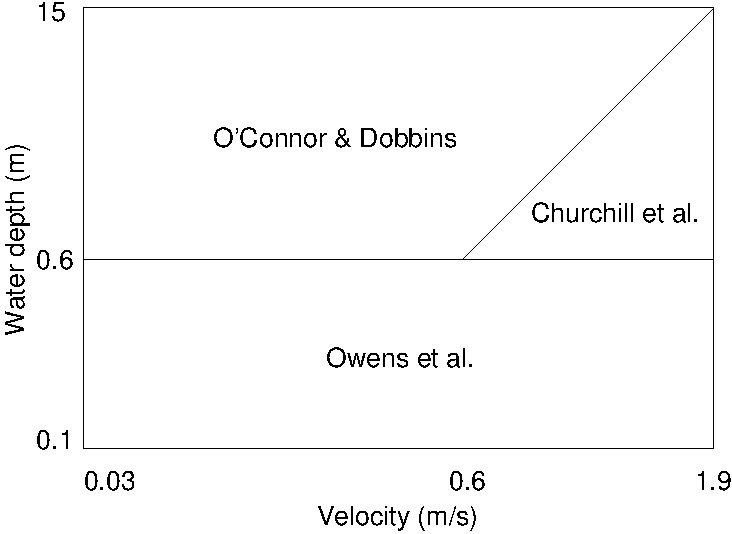
\includegraphics[scale=0.3]{graphics/validity_domain_reaeration_O2.png}
  \caption{Application areas of Owens et al., Churchill et al. and O'Connor
    and Dobbins formulae \cite{mccutcheon_wq_1989}.}
  \label{validity_domain_reaeration}
\end{figure}

One option allows the user fixing a value for $k_2$.
Another option allows choosing one of the four formulae described above.
The value of $k_2$, valid at 20$^{\circ}$C, is adjusted according to the temperature as:

\begin{equation}
  k_2 = (k_2)_{20^{\circ}\rm{C}} (1.0241)^{T-20}.
\end{equation}

The oxygen concentration at saturation in the water $C_s$ can be determined
according to the water temperature (at 20$^{\circ}$C, $C_s$ = 9 mgO$_2$/l).
This is a parameter that must be known and can be calculated
if connected to a temperature module such as THERMIC.
Elmore and Hayes (cited in \cite{mccutcheon_wq_1989}) proposed the following formula
(with $T$ in $^{\circ}$C) for calculating $C_s$:

\begin{equation}
  C_s = 14.652 - 0.41022 T + 0.007991 T^2 - 7.7774.10^{-5}T^3.
\end{equation}

More recent models include a correction for atmospheric pressure and, in estuaries, for salinity.
However, we consider that we are far from estuarial conditions and the variations in pressure
entail insignificant variations in dissolved oxygen compared to those that we need.
Montgomery et al.'s equation (cited in \cite{mccutcheon_wq_1989})
only deviates from standard formulae by $ \pm $  0.02 mgO$_2$/l
between 0 and 50$^{\circ}$C when there is negligible salinity.

\begin{equation}
  C_s = \frac{468}{31.6+T}.
\end{equation}

The model allows choosing either a fixed $C_s$ value given
by the user or by one of the two formulae described above.\\

\subsubsection{Reaeration due to weirs (not used at the moment in WAQTEL)}

A weir can provide between 1 and 3 mg/l of dissolved oxygen \cite{mccutcheon_wq_1989}.
The ratio $r$ is defined by the relationship $$r = \frac{C_s-C_u}{C_s-C_d},$$

with $C_u$ = oxygen concentration upstream of weir,
$C_d$ = oxygen concentration downstream of weir.
The knowledge of $C_u$ and $r$  enables calculating $C_d$.
$C_d$ is directly applied.
This term therefore is not treated as a source.
The rate $r$ can be determined empirically
\cite{mccutcheon_wq_1989}: e.g.,

\begin{equation}
  r = 1 + 0.5 a b \Delta h \quad \rm{(Gameson)},
\end{equation}

\begin{equation}
  r = 1+ 0.36 a b (1+0.046 T) \Delta h \quad \rm{(Gameson~et~al.)},
\end{equation}

\begin{equation}
  r = 1 + 0.69 \Delta h (1 - 0.11 \Delta h) (1 +0.046 T) \quad \rm{(Water~Research~Laboratory)},
\end{equation}

\begin{equation}
  r = 1 + 0.38 a b  \Delta h (1 - 0.11 \Delta h) (1 +0.046 T),
  \quad \rm{(Water~Research~Laboratory)}
\end{equation}

with $a$ = measure of water quality (= 0.65 for highly polluted streams,
= 1.8 for clear streams),
$b$ = characteristic parameter of the weir,
$\Delta h$ = water level difference between upstream and downstream of the weir.
The following Table gives $b$ values for different weirs \cite{mccutcheon_wq_1989}:\\

\begin{table}[H]
 			\centering
\begin{tabular}{p{3.0in}p{3.0in}}
\hline
%row no:1
\multicolumn{1}{|p{3.0in}}{Type of weir} & 
\multicolumn{1}{|p{3.0in}|}{$b$} \\
\hline
%\hhline{--}
%row no:2
\multicolumn{1}{|p{3.0in}}{flat broad-crested regular step} & 
\multicolumn{1}{|p{3.0in}|}{0.7} \\
\hline
%\hhline{--}
%row no:3
\multicolumn{1}{|p{3.0in}}{flat broad-crested irregular step} & 
\multicolumn{1}{|p{3.0in}|}{0.8} \\
\hline
%\hhline{--}
%row no:4
\multicolumn{1}{|p{3.0in}}{flat broad-crested vertical face} & 
\multicolumn{1}{|p{3.0in}|}{0.8} \\
\hline
%\hhline{--}
%row no:5
\multicolumn{1}{|p{3.0in}}{flat broad-crested straight slope face} & 
\multicolumn{1}{|p{3.0in}|}{0.9} \\
\hline
%\hhline{--}
%row no:6
\multicolumn{1}{|p{3.0in}}{flat broad-crested curved face} & 
\multicolumn{1}{|p{3.0in}|}{0.75} \\
\hline
%\hhline{--}
%row no:7
\multicolumn{1}{|p{3.0in}}{round broad-crested curved face} & 
\multicolumn{1}{|p{3.0in}|}{0.6} \\
\hline
%\hhline{--}
%row no:8
\multicolumn{1}{|p{3.0in}}{sharp-crested straight slope face} & 
\multicolumn{1}{|p{3.0in}|}{1.05} \\
\hline
%\hhline{--}
%row no:9
\multicolumn{1}{|p{3.0in}}{sharp-crested vertical face} & 
\multicolumn{1}{|p{3.0in}|}{0.8} \\
\hline
%\hhline{--}
%row no:10
\multicolumn{1}{|p{3.0in}}{sluice gates with submerged discharge} & 
\multicolumn{1}{|p{3.0in}|}{0.05} \\
\hline
%\hhline{--}

\end{tabular}
\end{table}

In the model, $r$ can be either a fixed value given by the user or
calculated by one of the 4 formulae previously described.\\

\section{Organic load}

The organic load $L$ (in mgO$_2$/l) is a variable evolving over time
from an initial condition according to a 1$^{\rm{st}}$ order law:

\begin{equation}
  F([L]) = -k_1 [L],
\end{equation}

where $k_1$ is the kinetic degradation constant of the organic load (d$^{-1}$).
It is a parameter of the model.
In the O$_2$ model, the organic load $L$ is considered to be an independent variable.

\section{Ammonia load}

Also consuming oxygen, the variable ammonia load NH$_4$ (in mgH$_4$/l) follows
a 1$^{\rm{st}}$ order decay law

\begin{equation}
  F([NH_4]) = -k_4 [NH_4],
\end{equation}

where $k_4$ the kinetic constant of nitrification (d$^{-1}$),
a parameter of the model.
In the O$_2$ model, the ammonia load is considered to be an independent variable.\\

\section{Solved equation in 2D}

The concentration of dissolved oxygen [O$_2$] (in mgO$_2$/l) changes
according to the effect of sources:

\begin{equation}
  F([O_2]) = k_2 (C_s - [O_2]) -k_1 [L] - k_4 [NH_4] + P - R - \frac{BEN_T}{h}.
\end{equation}

Using the terminology and notations of section \ref{waq_models}
and setting $C_1$ = [O$_2$], $C_2$ = [L] and $C_3$ = [NH$_4$],
the matrices [$ \lambda $] and [$ \mu $]
%containing the coefficients $\lambda_i^j$ and $ \mu_i^j$
are written as:\\

$$  [\lambda] = \frac{1}{86400}
  \begin{pmatrix}
    -k_2 & -k_1  & -k_4 \\
     0   & -k_1  & 0    \\
     0   &  0    & -k_4
  \end{pmatrix}
$$

$$
  [\mu] =
  \begin{pmatrix}
     0  & 0 & 0 \\
     0  & 0 & 0 \\
     0  & 0 & 0
  \end{pmatrix}
$$

(Note: Division by 86,400 scales down the time to one second).\\

The only non-zeros terms $ \lambda_1^0$ and $ \mu_1^0$ are:

\begin{equation}
  \lambda_1^0 = \frac{k_2 C_s + P - R}{86400},
\end{equation}

\begin{equation}
  \mu_1^0 = -\frac{BEN_T}{86400}.
\end{equation}

\section{Solved equation in 3D}

The concentration of dissolved oxygen [O$_2$] (in mgO$_2$/l) changes
according to the effect of sources:

\begin{equation}
  F([O_2]) = k_2 (C_s - [O_2]) -k_1 [L] - k_4 [NH_4] + P - R  - \frac{BEN_T}{\Delta z}.
\end{equation}

with $\Delta z$ half height of the bottom layer cells.

Using the terminology and notations of section \ref{waq_models}
and setting $C_1$ = [O$_2$], $C_2$ = [L] and $C_3$ = [NH$_4$],
the matrices [$ \lambda $] and [$ \mu $]
%containing the coefficients $\lambda_i^j$ and $ \mu_i^j$
are written as:\\

$$  [\lambda] = \frac{1}{86400}
  \begin{pmatrix}
    -k_2 & -k_1  & -k_4 \\
     0   & -k_1  & 0    \\
     0   &  0    & -k_4
  \end{pmatrix}
$$

$$
  [\mu] =
  \begin{pmatrix}
     0  & 0 & 0 \\
     0  & 0 & 0 \\
     0  & 0 & 0
  \end{pmatrix}
$$

(Note: Division by 86,400 scales down the time to one second).\\

The only non-zeros terms $ \lambda_1^0$ and $ \mu_1^0$ are:

\begin{equation}
  \lambda_1^0 = \frac{k_2 C_s + P - R - \frac{BEN_T}{\Delta z}}{86400},
\end{equation}

\begin{equation}
  \mu_1^0 = 0.
\end{equation}


%----------------------------------------------------------------------------------------
%       CHAPTER : THERMIC module
%----------------------------------------------------------------------------------------

\chapter{The THERMIC module}
\label{subs:therm:mod}
For a majority of water quality processes, the interaction with atmosphere is a key parameter.
The THERMIC module is activated by setting \telkey{WATER QUALITY PROCESS} = 11.
The neighboring conditions are taken into account through a meteorological file
like the one described in section \ref{subs:meteo:file}.
It is important to underline that the data contained in this file
can vary depending on the considered case.
The subroutine \telfile{meteo.f} can be edited by the user to customize it to his specific model.

Before version 7.0, heat exchange between water and atmosphere could have been
done with a linearised formula of the balance of heat exchange fluxes at the
free surface in \telemac{3D}. An example of an exchange with a constant atmosphere temperature
and a constant sea salinity was given as standard (as comments) through a
direct programming in the \telfile{BORD3D} subroutine.\\

A much more elaborated model has been introduced in \waqtel for 2D and 3D.

The evolution of temperature of water is tightly linked to heat fluxes through the free surface.
These fluxes (in W/m$^2$) are of 5 natures:

\begin{itemize}
\item solar radiation or sun ray flux $RS$,
\item atmospheric radiation flux $RA$,
\item water radiation or free surface radiation flux $RE$,
\item latent heat or heat flux due to advection $CV$,
\item sensitive heat of conductive origin or heat flux due to evaporation $CE$.
\end{itemize}

The final balance of (surface) source terms is given by:
\[S_{surf}=RS+RA-RE-CV-CE\]
We will give a brief description for each of these terms, for more details see \cite{El-Kadi2012}.
This surface source term is treated explicitly in \telemac{2D},
the following term is added in the explicit source term of advection-diffusion equation
of tracer$\frac{S_{surf}}{\rho C_pH}$.\\

There is a distinction done in 3D compared to 2D:
whereas the long wave radiation (atmospheric radiation $RA$) is absorbed in
the first centimetres of the water column, the short wave radiation (solar
radiation $RS$) penetrates the water column. Evaporation is calculated in 3D.

The choice of the heat exchange model can be done with the keyword
\telkey{ATMOSPHERE-WATER EXCHANGE MODEL} in the \waqtel steering file
(default value = 0: no exchange
model). Value 1 will use with the linearised formula at the free surface,
whereas value 2 will use with the model with complete balance.

These calculations require additional meteo data which may vary in time
in an expected format, rather defined
in the \telkey{ASCII ATMOSPHERIC DATA FILE} of the \telemac{3D} steering file,
see the example "heat\_exchange".

Since release v8.2 the format of the \telkey{ASCII ATMOSPHERIC DATA FILE} is
flexible with respect to the order of columns (but with the mandatory convention
for data names with the shortnames listed in \ref{subs:meteo:file}).

If not filling the necessary variables
(in 3D: wind velocities, air temperature, atmospheric pressure, cloud cover,
rainfall, relative humidity;
 in 2D: wind velocities, air temperature, atmospheric pressure, cloud cover,
rainfall, solar radiation, saturated vapour pressure),
the missing variables are considered constant along the whole computation and
their values are set by associated keywords values
(\telkey{WIND VELOCITY ALONG X}, \telkey{WIND VELOCITY ALONG Y}, or
\telkey{SPEED AND DIRECTION OF WIND} for wind velocity,
\telkey{VALUE OF ATMOSPHERIC PRESSURE} for atmospheric pressure,
\telkey{RAIN OR EVAPORATION IN MM PER DAY} for rainfall,
\telkey{AIR TEMPERATURE}, \telkey{CLOUD COVER}, \telkey{RELATIVE HUMIDITY},
\telkey{SOLAR RADIATION}, \telkey{VAPOROUS PRESSURE}).

%The format may be changed but the user has to change the
%implementation of the reading and the interpolation of the meteorological data.

When using the complete module, evaporation is calculated by \telemac{3D}, but
the user has to provide rainfall data with units homogeneous with length over
time.

The main developments of this module are implemented in the module
\telfile{EXCHANGE\_WITH\_ATMOSPHERE} in 3D and in the \telfile{CALCS2D\_THERMIC} in 2D.


\section{Sun ray flux RS}

Sun ray flux is simply provided in the \telkey{ASCII ATMOSPHERIC DATA FILE} in 2D.
In a majority of cases, when no measurements are available,
this flux is estimated using the method of Perrin \& Brichambaut (\cite{El-Kadi2012}),
which uses the cloud cover of the sky that varies during the day (function of time).
So far, this flux is considered constant in space.

Since release 8.2, solar radiation or sun ray can be either read in the 
\telkey{ASCII ATMOSPHERIC DATA FILE} or computed by \waqtel in 3D.
To read it in the meteo file, the keyword
\telkey{SOLAR RADIATION READ IN METEO FILE} is to be activated (default = NO,
i.e. it is computed by \waqtel in 3D).
Moreover, an additional column is to be written with the shortname RAY3
as headline of the column.

For more real cases, the user is invited to use the ``heat exchange'' module
(in folder sources/telemac3d).
A sun ray flux varying in space, common between \telemac{2D} and \telemac{3D} will be implemented in next releases.

In 3D, examples of solar radiation penetration in the water $RS$ are given in the
\telfile{CALCS3D\_THERMICV} subroutine. Two laws are suggested: the first one
uses the \emph{in situ} measurements of Secchi length and is
recommended if available; the second one uses two exponential laws that may be
difficult to calibrate and require an estimation of the type of water from
turbidity.
An example of the a double exponential law is commented.
A similar law as Atkins formula with Secchi length (see BIOMASS module) can also be
used with light extinction coefficient directly given with the keyword
\telkey{LIGHT EXTINCTION COEFFICIENT} as soon as
\telkey{METHOD OF COMPUTATION OF RAY EXTINCTION COEFFICIENT} is set to 3.

The type of sky related to the luminosity of the site has to be chosen
with respect to the considered area, with the \waqtel keyword
\telkey{LIGHTNESS OF THE SKY} (1: very pure sky, 2: mean pure sky which is default
or 3: industrial zone sky) in 3D.


\section{Atmospheric radiation RA}

The atmospheric radiation $RA$ is estimated with meteorological
data collected at the ground level.
It takes into account energy exchanges with the ground, water
(and energy) exchanges with the underground, etc.\\

In 2D, $RA$ is estimated mainly by the air temperature, like:
\begin{equation*}
RA=e_{air}\sigma\left(T_{air}+273.15 \right)^4\left(1+k\left(\frac{c}{8}\right)^2 \right),
\end{equation*}
where:
\begin{itemize}
\item $e_{air}$ is a calibrating coefficient given by the keyword
  \telkey{COEFFICIENTS FOR CALIBRATING ATMOSPHERIC RADIATION} (default = 0.97),
\item $\sigma$ is the constant of Stefan-Boltzmann (= 5.67.10$^{-8}$ Wm$^{-2}$K$^{-4}$),
\item $T_{air}$ is air temperature given in the \telkey{ASCII ATMOSPHERIC DATA FILE},
\item $c$ = cloudiness (octas), given in the atmospheric data file
(WARNING: in \khione, it is given in tenths),
\item $k$ is the coefficient that represents the nature and elevation of clouds,
it has a mean value of 0.2 and can be changed with the keyword
\telkey{COEFFICIENT OF CLOUDING RATE}.
To simplify calculations, an average value of $k$ = 0.2 is usually taken in 2D
(but default value = 0.17 like in 3D since release 8.2,
old default value was 0.2 until release 8.1).
However, it varies like indicated in Table \ref{tab:kcloud}.
\end{itemize}

\begin{table}
  \centering
  \begin{tabular}{|l|c|}
     \hline
     Type of cloud & $k$ \\
     \hline \hline
     Cirrus & 0.04 \\
     Cirro-stratus & 0.08 \\
     Altocumulus & 0.17 \\
     Altostratus & 0.2 \\
     Cumulus & 0.2 \\
     Stratus & 0.24\\
     \hline
   \end{tabular}
  \caption{Values of $k$ depending on cloud type}\label{tab:kcloud}
\end{table}

In 3D, clouds and albedo at
the free surface determine the atmospheric radiation $RA$ penetrating the water:
\begin{equation*}
RA = (1-alb_{lw}) e_{air}\sigma(T_{air}+273.15)^{4}(1+k . \left( \frac{C}{8} \right)^{2}),
\end{equation*}
where:
\begin{itemize}
\item $alb_{lw}$ = 0.03 is the water albedo for long radiative waves
  (common value used in the literature \cite{imerito_dyresm_2007},
  \cite{henderson-sellers_energy_balance_1986}),
  (1-$alb_{lw}$) is equal to the calibrating coefficient given by the keyword
  \telkey{COEFFICIENTS FOR CALIBRATING ATMOSPHERIC RADIATION} (default = 0.97,
  hence $alb_{lw}$ = 0.03 as default value),
%\item $T_{air}$ ($^{\circ}$C) is the air temperature,
\item $e_{air}$ is the air emissivity (= $0.937.10^{-5}(T_{air}+273.15)^{2}$
if using Swinbank formula, default option),
\item $\sigma= 5.67.10^{-8}~\mathrm{{W.m^{-2}.K^{-4}}}$ is Stefan-Boltzmann's constant,
\item $C$ is the nebulosity (octas). Some meteorological services such as
M\'{e}t\'{e}o France provide this data in octas, it needs to be converted
into tenths, hence the division by 8 in the formula,
(WARNING: in \khione, it is given in tenths),
\item $k$ (dimensionless) is a parameter characterising the type of
cloud. In practise, it is difficult to know the type of cloud during the
period of simulation and a mean value of 0.17 is often used \cite{tva_heat_1972},
\cite{imerito_dyresm_2007}.
This is the new default value for the keyword
\telkey{COEFFICIENT OF CLOUDING RATE} since release 8.2.
Other choices are possible
%hard-coded in 3D but other choices are possible
(see the table \ref{tab:kcloud}).
%and can be changed in the module
%\telfile{EXCHANGE\_WITH\_ATMOSPHERE}.
\end{itemize}

When coupling \waqtel with \telemac{3D}, the \telkey{FORMULA OF ATMOSPHERIC RADIATION}
can be changed:
\begin{itemize}
\item 1: Idso and Jackson (1969),
\item 2: Swinbank (1963) which is the default formula,
\item 3: Brutsaert (1975),
\item 4: Yajima Tono Dam (2014).
\end{itemize}

The formulae in 2D and 3D are almost the same with few differences.


\section{Free surface radiation RE}

The available water is assumed to behave like a grey body.
Radiation generated by this grey body through the free surface is given by:
\begin{equation*}
RE = e_{water}\sigma\left(T_{water}+273.15 \right)^4,
\end{equation*}
where:
\begin{itemize}
\item $T_{water}$ is the mean water temperature in ${}^\circ$C.
$T_{water}$ is given by the keyword \telkey{WATER TEMPERATURE} (default 7${}^\circ$C),
\item $e_{water}$ can be seen as a calibration coefficient which depends on the nature
of the site and obstacles around it.
This coefficient is given with
\telkey{COEFFICIENTS FOR CALIBRATING SURFACE WATER RADIATION} (default 0.97).
For instance, for a narrow river with lots of trees on its banks,
$e_{water}$ is around 0.97, for large rivers or lakes it is about 0.92.
\end{itemize}


\section{Advection heat flux CV}

This flux (also called sensitive heat flux) is estimated empirically:
\begin{equation*}
CV=\rho_{air}C_{p_{air}}f(V)\left(T_{water}-T_{air} \right),
\end{equation*}
where:
\begin{itemize}
  \item $\rho_{air}$ is the air density given by
${\rho }_{air}=\ \frac{100\ P_{atm}}{\left(T_{air}+273.15\right)287}$
where $P_{atm}$ is the atmospheric pressure,
introduced in the \telkey{ASCII ATMOSPHERIC DATA FILE} or using the keyword
\telkey{VALUE OF ATMOSPHERIC PRESSURE} (default 100,000~Pa),
this is a keyword of \telemac{2D} and \telemac{3D},
\item $C_{p_{air}}$ is the air specific heat (J/kg${}^\circ$C)
  given by \telkey{AIR SPECIFIC HEAT} (default 1,005),
\item $f(V)$ is a function of the wind velocity $V$:
  \begin{itemize}
  \item in 2D: $f(V) = a+bV$,
  \item in 3D: $f(V) = b(1+V)$ for wind velocity at 2~m high
    or $f(V) = a+bV$ for wind velocity at 10~m high,
    depending on user's choice,
  \end{itemize}
\item $V$ is the wind velocity (m/s),
\item $a$, $b$ are empirical coefficients to be calibrated in 2D and in 3D (only $a$ if one single calibrating coefficient).
Their values are very close to 0.0025, but they can be changed
using \telkey{COEFFICIENTS OF AERATION FORMULA} (default = (0.002, 0.0012)).
\end{itemize}

Because the site of a study may not be equipped with local wind measurements
and these kinds of data are available at a different location, possibly far
from the studied site, a wind function is used.
In 3D, this can be a linear function with
a single coefficient of calibration $b:f(U_{2}) = b(1+U_{2}$) where $U_{2}$ is
the wind velocity at 2~m high.

To get the wind velocity at 2~m high from classical wind data at 10~m high, a
roughness length of ${z}_{0}~=~0.0002$~m has been chosen in the code,
that leads to $U_{2} \approx 0.85 U_{10}$. This value
of 0.85 (or the roughness length) may be changed by the user if needed.\\

In 3D, except for the coefficient to model the penetration of solar radiation in the
water column,
and if there is only one single calibrating coefficient,
the parameter $b$ that appears in the wind function is the
single calibration parameter of this module. Its value is given by the keyword
\telkey{COEFFICIENT TO CALIBRATE THE ATMOSPHERE-WATER EXCHANGE MODEL}
in the \waqtel steering file (default
value = 0.0025 but recommended values are between 0.0017 and 0.0035). This
keyword is both used for the linearised formula at the free surface and the
model with complete balance (values 1 and 2 for the keyword
\telkey{ATMOSPHERE-WATER EXCHANGE MODEL} in the \waqtel steering file).

Since release 8.2, the user can define a wind function depending on 2 coefficients
by filling in the \telkey{COEFFICIENTS OF AERATION FORMULA}
(not letting the default values).
These 2 coefficients are then taken into account rather the 1 single coefficient
if using \telkey{ATMOSPHERE-WATER EXCHANGE MODEL} = 2.
Contrary to the wind function with one single coefficient to calibrate where
wind velocity is taken at 2~m high, the wind function with 2 coefficients
uses wind velocity taken at 10~m high.


\section{Evaporation heat flux CE}

The evaporative heat flux $CE$ (also called latent heat flux)
is given by the following empirical formula:
\begin{equation*}
CE = L(T_{water})\rho_{air}f(V) \left(H^{sat}-H \right)
\end{equation*}
where:
\begin{itemize}
\item $L(T_{water})$ = 2,500,900 - 2,365.$T_{water}$ is the vaporization latent heat (J/Kg),
\item $f(V)$ is a function of the wind velocity $V$:
  \begin{itemize}
  \item in 2D: $f(V) = a+bV$,
  \item in 3D: $f(V) = b(1+V)$ for wind velocity at 2~m high
    or $f(V) = a+bV$ for wind velocity at 10~m high,
    depending on user's choice,
  \end{itemize}
\item $V$ is the wind velocity (m/s),
\item $H^{sat}=\frac{0.622P^{sat}_{vap}}{P_{atm}-0.378P^{sat}_{vap}}$
is the air specific moisture (humidity) at saturation (kg/kg),
\item $H = \frac{0.622P_{vap}}{P_{atm}-0.378P_{vap}}$ is the air specific humidity (kg/kg),
\item $P_{vap}$ is the partial pressure of water vapour in the air (hPa)
which is given in the \telkey{ASCII ATMOSPHERIC DATA FILE},
\item $P^{sat}_{vap}$ is the partial pressure of water vapour at saturation (hPa) which is estimated with:
\begin{equation*}
P^{sat}_{vap} = 6.11 \exp \left(\frac{17.27T_{water}}{T_{water}+237.3} \right).
\end{equation*}
\end{itemize}

When $H{}^{sat} < H$, the atmospheric radiation $RA$ is corrected by multiplying it with 1.8.


%----------------------------------------------------------------------------------------
%       CHAPTER : BIOMAS module
%----------------------------------------------------------------------------------------

\chapter{BIOMASS Module}

The BIOMASS module is a water quality module which allows the calculation of algal biomass.
It estimates the extent of vegetal colonization in terms of various parameters:
sunlight, water temperature, fertilization degree, water renewal ratio,
water turbidity and toxicity \cite{gosse_biomass_1983}.
The BIOMASS module is activated by setting \telkey{WATER QUALITY PROCESS} = 3.

It takes into account five tracers:

\begin{itemize}
\item phytoplankton biomass PHY,
\item the principal nutrients influencing its production (phosphorus, nitrogen)
  as well as the associated mineral forms, namely:

\begin{itemize}
\item dissolved mineral phosphorus assimilable by phytoplankton PO$_4$,
\item degradable phosphorus not assimilable by phytoplankton POR,
\item dissolved mineral nitrogen assimilable by phytoplankton NO$_3$,
\item degradable nitrogen not assimilable by phytoplankton NOR.
\end{itemize}
\end{itemize}

These variables are all expressed in mg/l except biomass that is expressed in $\mu$g(Chlorophyl a)/l.\\

The following sections explain the internal source terms.

For more details about the theory of the O2 module,
the reader can refer to the \waqtel technical manual.


\section{Processes represented}

The bottom and the processes that occur there are not modeled in the BIOMASS model.
Deposition is only represented by the deposition flux and,
once organic matter is deposited,
it no longer appears in the equations and can no longer be resuspended.
These deposition fluxes therefore correspond to a definitive loss of mass.


\section{Phytoplankton}

\subsection{Algal growth}

The algal growth rate $CP$ (d$^{-1}$) is given by:

\begin{equation*}
  CP = C_{max} RAY g_1 LNUT \alpha_1,
\end{equation*}

with $C_{max}$ = maximum algal growth rate at 20$^{\circ}$C;
one can set its value with the keyword \telkey{MAXIMUM ALGAL GROWTH RATE AT 20C} (default = 2).
$RAY$ represents the effect of sunlight on algal growth,
this dimensionless parameter ranges between 0 and 1.
$g_1 = T/20$ represents the effect of temperature on algal growth.
$LNUT$ represents the effects of phosphoric and nitric nutrients on algal growth.
$\alpha_1$ = water toxicity coefficient for algae ($\alpha_1$ = 1 in the absence of toxicity),
this last value can be chosen with the 1$^{\textrm{st}}$ value of the keyword
\telkey{ALGAL TOXICITY COEFFICIENTS} (default = 1).\\
$RAY$ is calculated by the Smith formula averaged over the vertical:

\begin{equation*}
  RAY = \frac{1}{k_e h} \log \left( \frac{I_0 + \sqrt{IK^2+I_0^2} }{ I_h + \sqrt{IK^2+I_h^2} }  \right),
\end{equation*}

where $k_e$ is the extinction coefficient of solar rays in water.
The formula to compute $k_e$ can be chosen with the keyword
\telkey{METHOD OF COMPUTATION OF RAY EXTINCTION COEFFICIENT} (default = 1):
\begin{itemize}
  \item 1: Atkins formula, it is calculated either by the Secchi depth $Z_s$
(keyword \telkey{SECCHI DEPTH}, default = 0.9~m, if it is a constant value),
    %$k_e$ = 1.7/$Z_s$,
  \item 2: the Moss relation: $k_e$ = $k_{pe}$+$ \beta $ [PHY] if $Z_s$ is unknown,
    where $k_{pe}$ is the coefficient of vegetal turbidity without phytoplankton
    provided with the keyword \telkey{VEGETAL TURBIDITY COEFFICIENT WITHOUT PHYTO}
    (default = 0~m$^{-1}$)
    and $\beta$ the Moss coefficient ($\beta \approx$ 0.015),
  \item 3: constant given by the user with the keyword
    \telkey{LIGHT EXTINCTION COEFFICIENT} (default = 0.2~m$^{-1}$).
\end{itemize}

$IK$ is a calibrating parameter
associated to the keyword \telkey{PARAMETER OF CALIBRATION OF SMITH FORMULA}
(default = 120~W/m$^2$) of an order of magnitude 100.
$I_0$ is the flux density of solar radiation on the surface
which can be set with the keyword \telkey{SUNSHINE FLUX DENSITY ON WATER SURFACE}
(default = 0~W/m$^2$)
and $I_h$ is the flux density of solar radiation at the bed bottom (W/m$^2$), calculated as:

\begin{equation*}
  I_h = I_0 \exp (-k_e h).
\end{equation*}

$LNUT$ is calculated by the formula:

\begin{equation*}
  LNUT = \min \left( \frac{[PO_4]}{KP+[PO_4]}, \frac{[NO_3]}{KN+[NO_3]} \right),
\end{equation*}

with $KP$ = phosphate half-saturation constant
set with the keyword \telkey{CONSTANT OF HALF-SATURATION WITH PHOSPHATE}
(default = 0.005 mgP/l),
and $KN$ = nitrate half-saturation constant
set with the keyword \telkey{CONSTANT OF HALF-SATURATION WITH NITROGEN}
(default = 0.03~mgN/l).\\

\subsection{Algal disappearance}

The algal disappearance rate $DP$ (d$^{-1}$) is given as:

\begin{equation*}
  DP = (RP+MP) g_2,
\end{equation*}

with $RP$ = algal biomass respiration rate at 20$^{\circ}$C
given by the keyword \telkey{RESPIRATION RATE OF ALGAL BIOMASS}
(default = 0.05~d$^{-1}$),
$MP$ = algal biomass disappearance rate at 20$^{\circ}$C (d$^{-1}$).
$g_2 = T/20$ represents the effect of temperature on algal disappearance.
$MP$ is given by the following relation:

\begin{equation*}
  MP = M_1 + M_2 [PHY] + \alpha_2,
\end{equation*}

with $M_1$ and $M_2$ = algal mortality coefficients at 20$^{\circ}$C
which can be set with the keyword
\telkey{COEFFICIENTS OF ALGAL MORTALITY AT 20C} (default = (0.1;0.003)),
$\alpha_2$ = water toxicity coefficient for algae,
this last value can be chosen with the 2$^{\textrm{nd}}$ value of the keyword
\telkey{ALGAL TOXICITY COEFFICIENTS} (default = 0).

\section{Nitric and phosphoric nutrients}

The following physical and biochemical parameters are used
to describe the processes influencing the evolution of nitric and phosphoric nutrients:

\begin{itemize}
\item \telkey{PROPORTION OF PHOSPHORUS WITHIN PHYTO CELLS}
  for the average proportion of phosphorus in the cells of living phytoplankton $fp$ (0.0025~mgP/$\mu$gChlA),
\item \telkey{PERCENTAGE OF PHOSPHORUS ASSIMILABLE IN DEAD PHYTO}
  for the proportion of directly assimilable phosphorus in dead phytoplankton $dtp$ (default = 0.5),
\item \telkey{RATE OF TRANSFORMATION OF POR TO PO4}
  for transformation rate of POR into PO$_4$ through bacterial mineralization $k_1$ (default = 0.03~d$^{-1}$),
\item \telkey{RATE OF TRANSFORMATION OF NOR TO NO3}
  for transformation rate of NOR into NO$_3$ through heterotrophic
  and autotrophic bacterial mineralization $k_2$ (default = 0~d$^{-1}$),
\item \telkey{PROPORTION OF NITROGEN WITHIN PHYTO CELLS}
  for the average proportion of directly assimilable nitrogen in living phytoplankton $fn$ (0.0035~mgN/$\mu$gChlA),
\item \telkey{PERCENTAGE OF NITROGEN ASSIMILABLE IN DEAD PHYTO}
  for the proportion of directly assimilable nitrogen in dead phytoplankton $dtn$ (default = 0.5),
\item $F_{POR}$: deposition flux of non-algal organic phosphorus (g/m$^2$/s).
  $F_{POR} = W_{POR} [POR]$,
  $W_{POR}$ is the sedimentation velocity of non-algal organic phosphorus
  given by the keyword \telkey{SEDIMENTATION VELOCITY OF ORGANIC PHOSPHORUS}
  (default = 0~m/s),
\item $F_{NOR}$: deposition flux of non-algal organic nitrogen (g/m$^2$/s).
  $F_{NOR} = W_{NOR} [NOR]$, $W_{NOR}$ is the sedimentation velocity of non-algal organic nitrogen
  given by the keyword \telkey{SEDIMENTATION VELOCITY OF NON ALGAL NITROGEN}
  (default = 0~m/s).
\end{itemize}

\begin{WarningBlock}{Warning:}
Since release 8.5 and as long as no good solution to implement the treatment of
sedimentation velocities (N and P) is found, this treatment has
been commented in the source code so that it is not possible to take them into
account \emph{in 3D}.
Thus keywords \telkey{SEDIMENTATION VELOCITY OF ORGANIC PHOSPHORUS} and
\telkey{SEDIMENTATION VELOCITY OF NON ALGAL NITROGEN} are not taken into account.
The behaviour is as they would be let to default value = 0~m/s.
\end{WarningBlock}


%----------------------------------------------------------------------------------------
%       CHAPTER : EUTRO module
%----------------------------------------------------------------------------------------

\chapter{EUTRO Module}

The EUTRO module describes the oxygenation of a river and
is not restricted to modeling reaeration and the global oxidizable load.
It takes into account the effect of planktonic photosynthesis,
models the nitric and phosphoric nutrients and their effect
on phytoplankton (\cite{gosse_doubs_1989} and \cite{gosse_doubs_1983}).
It is activated by setting \telkey{WATER QUALITY PROCESS} = 5.\\

This module is a combination of the O$_2$ and BIOMASS modules,
except for a more precise treatment of some parameters,
taking into account the ammonia load in exchanges between nitrogen and phytoplankton,
and of phytoplankton in the calculation of photosynthesis.
More sophisticated than the O$_2$ module, the EUTRO module requires setting
the values of 28 parameters (excluding the parameterization of the weirs).\\

The EUTRO module involves 8 tracers:

\begin{itemize}
\item dissolved oxygen O$_2$,
\item phytoplankton biomass (which consumes oxygen through photosynthesis) PHY,
\item the main elements influencing their production
  (phosphorus, nitrogen, ammonia load, organic load)
  as well as the mineral forms associated with phosphorus and nitrogen:
\begin{itemize}
\item dissolved mineral phosphorus assimilable by phytoplankton PO$_4$,
\item degradable phosphorus non-assimilable by phytoplankton POR,
\item dissolved mineral nitrogen assimilable by phytoplankton NO$_3$,
\item ammonia load assimilable by phytoplankton (and consuming oxygen) NH$_4$,
\item degradable nitrogen non-assimilable by phytoplankton NOR,
\item organic load (consuming oxygen) L.
\end{itemize}
\end{itemize}

These variables are expressed in mg/l, except for biomass which is expressed in $\mu$g (Chlorophyll a)/l.\\

For more details about the theory of the EUTRO module,
the reader can refer to the \waqtel technical manual.


\section{Processes represented}

%Figure \ref{ecosyst_scheme} presents the various phenomena modeled\ by the EUTRO model.\\

The following parts show the parameters used and detail internal sources for each of the 8 tracers studied.\\

As with the BIOMASS module, sediment transport and resulting bed geometry changes
are not modeled in the EUTRO module
(only a deposition flux is taken into account and the quantities deposited no longer appear in the equations).\\

%\begin{figure}[H]
%  \centering
%%  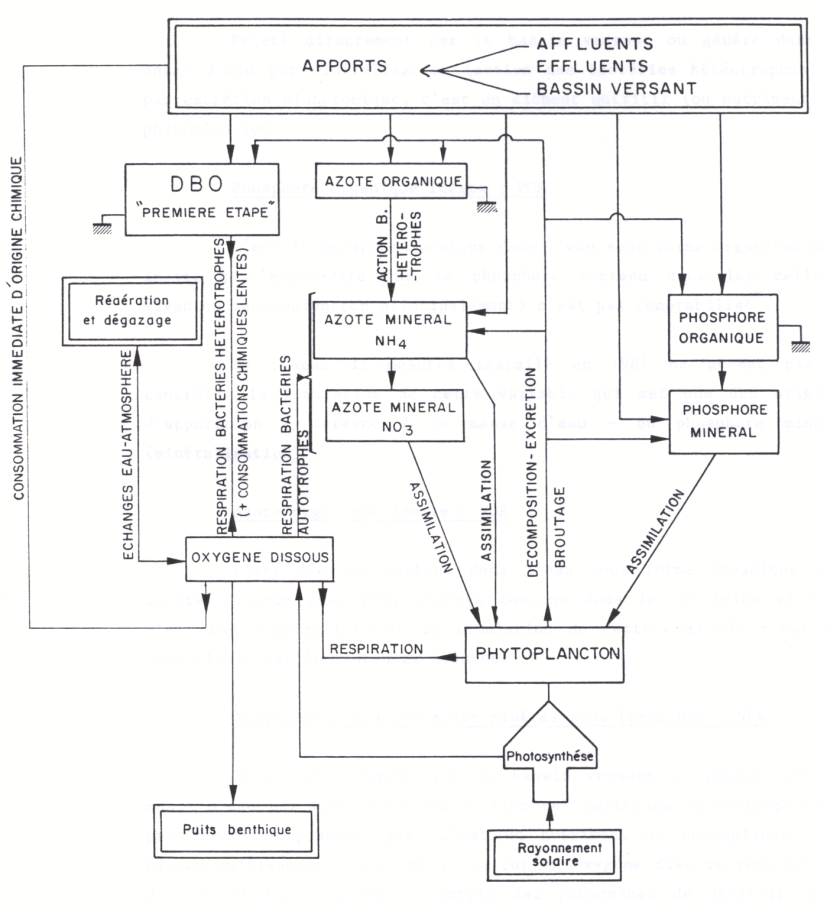
\includegraphics[scale=1.]{graphics/image38.png}
%  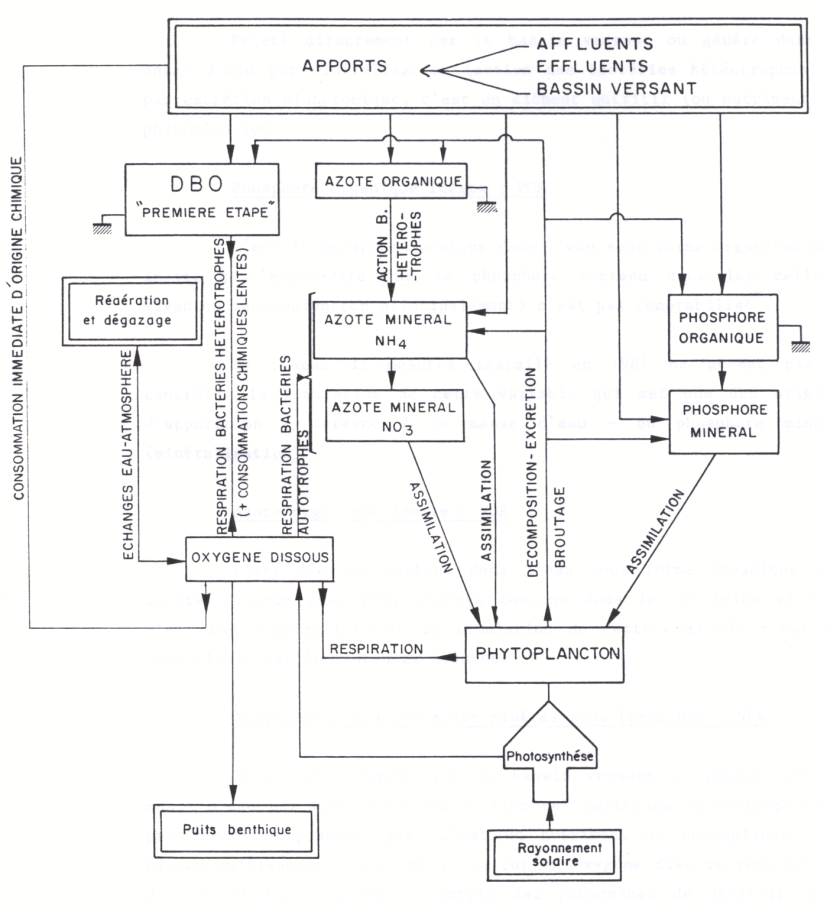
\includegraphics[width=3.76in,height=4.01in]{graphics/image38.png}
%  \caption{Schematic representation of the ecosystem modeled by the EUTRO module \cite{gosse_doubs_1989}.
%    Figure taken from \cite{elkadi_tracer_2012}.}
%  \label{ecosyst_scheme}
%\end{figure}

\section{Phytoplankton}

\subsection{Algal growth}

The algal growth rate $CP$ (d$^{-1}$) is given by
the exactly same equation as in BIOMASS module.
The parameters $C_{max}$
(\telkey{MAXIMUM ALGAL GROWTH RATE AT 20C}, default = 2),
$RAY$, $g_1$ and $\alpha_1$
(this last value can be chosen with the 1$^{\textrm{st}}$ value of the keyword
\telkey{ALGAL TOXICITY COEFFICIENTS}, default = 1 i.e. absence of toxicity)
are defined in the same way as in the BIOMASS module.

The parameters
\telkey{METHOD OF COMPUTATION OF RAY EXTINCTION COEFFICIENT} (default = 1 i.e.
Atkins formula with Secchi depth),
\telkey{VEGETAL TURBIDITY COEFFICIENT WITHOUT PHYTO} (default = 0~m$^{-1}$),
\telkey{PARAMETER OF CALIBRATION OF SMITH FORMULA} (default = 120~W/m$^2$),
\telkey{SUNSHINE FLUX DENSITY ON WATER SURFACE} (default = 0~W/m$^2$)
are still to be set as in BIOMASS.\\

The parameter representing the effects of phosphoric
and nitric nutrients on the algal growth $LNUT$ takes into account
the ammonia load assimilable by the phytoplankton NH$_4$ and is therefore defined by:

\begin{equation}
  LNUT = \min \left( \frac{[PO_4]}{KP+[PO_4]}, \frac{[NO_3]+[NH_4]}{KN+[NO_3]+[NH_4]} \right),
\end{equation}

with $KP$ half-saturation constant in phosphate
set with the keyword \telkey{CONSTANT OF HALF-SATURATION WITH PHOSPHATE}
(default = 0.005 mgP/l) as in BIOMASS,
and $KN$ half-saturation constant in nitrates
set with the keyword \telkey{CONSTANT OF HALF-SATURATION WITH NITROGEN}
(default = 0.03 mgN/l) as in BIOMASS.\\

\subsection{Algal disappearance}

The algal disappearance rate $DP$ (d$^{-1}$) is given
by the the same equation as in BIOMASS module.
\telkey{RESPIRATION RATE OF ALGAL BIOMASS}
(default = 0.05~d$^{-1}$) and the keyword
\telkey{COEFFICIENTS OF ALGAL MORTALITY AT 20C} (default = (0.1;0.003))
and \telkey{ALGAL TOXICITY COEFFICIENTS} (default = (1;0))
are still to be set as in BIOMASS.\\

The effect of temperature on algal disappearance
is represented by the function $g_2 = (1,050)^{T-20}$.

\section{Nitric and phosphoric nutrients}

The following physical and biochemical parameters are used to describe processes
influencing the evolution of nitric and phosphoric nutrients:

\begin{itemize}
\item \telkey{PROPORTION OF PHOSPHORUS WITHIN PHYTO CELLS}
  for the average proportion of phosphorus in the cells of living phytoplankton $fp$ (0.0025~mgP/$\mu$gChlA),
\item \telkey{PERCENTAGE OF PHOSPHORUS ASSIMILABLE IN DEAD PHYTO}
  for the proportion of directly assimilable phosphorus in dead phytoplankton $dtp$ (default = 0.5),
\item \telkey{RATE OF TRANSFORMATION OF POR TO PO4}
  for the transformation rate of POR into PO$_4$ through bacterial mineralization at 20$^{\circ}$C
  $k_{320}$ (default = 0.03~d$^{-1}$),
\item \telkey{RATE OF TRANSFORMATION OF NOR TO NO3}
  for the transformation rate of NOR into NO$_3$ through heterotrophic
  and autotrophic bacterial mineralization at 20$^{\circ}$C $k_{620}$ (default = 0~d$^{-1}$),
\item \telkey{PROPORTION OF NITROGEN WITHIN PHYTO CELLS}
  for the average proportion of directly assimilable nitrogen in living phytoplankton $fn$ (0.0035~mgN/$\mu$gChlA),
\item \telkey{PERCENTAGE OF NITROGEN ASSIMILABLE IN DEAD PHYTO}
  for the proportion of directly assimilable nitrogen in dead phytoplankton $dtn$ (default = 0.5),
\item \telkey{CONSUMED OXYGEN BY NITRIFICATION}
  for the quantity of oxygen consumed by nitrification $n$ (default = 5.2~mgO$_2$/mgNH$_4$),
\item \telkey{CONSTANT FOR THE NITRIFICATION KINETIC K520}
  for the kinetics of nitrification at 20$^{\circ}$C $k_{520}$ (default = 0.35~d$^{-1}$),
\item $F_{POR}$: deposition flux of non-algal organic phosphorus (g/m$^2$/s).
  $F_{POR} = W_{POR} [POR]$,
  $W_{POR}$ is the sedimentation velocity of non-algal organic phosphorus
  given by the keyword \telkey{SEDIMENTATION VELOCITY OF ORGANIC PHOSPHORUS}
  (default = 0~m/s),
\item $F_{NOR}$: deposition flux of non-algal organic nitrogen (g/m$^2$/s).
  $F_{NOR} = W_{NOR} [NOR]$, $W_{NOR}$ is the sedimentation velocity of non-algal organic nitrogen
  given by the keyword \telkey{SEDIMENTATION VELOCITY OF NON ALGAL NITROGEN}
  (default = 0~m/s).

\item $Rn$: proportion of nitrogen assimilated in the form of NH$_4$ = $\frac{[NH_4]}{[NH_4]+[NO_3]}$.
\end{itemize}

\section{Organic load}

The following physical and biochemical parameters are used to describe processes
influencing the evolution of the organic load ($L$):

\begin{itemize}
\item \telkey{CONSTANT OF DEGRADATION OF ORGANIC LOAD K120}
  for kinetic degradation constant for the organic load at 20$^{\circ}$C $k_{120}$
  (default = 0.35~d$^{-1}$),
\item $g_3 = (1.047)^{T-20}$: effect of temperature on the degradation of organic load,
\item $F_{LOR}$: deposition flux of the organic load (g/m$^2$/s) = $W_{LOR}$.[L],
  with $W_{LOR}$ the sedimentation velocity of the organic load
  given by the keyword \telkey{SEDIMENTATION VELOCITY OF ORGANIC LOAD}
  (default = 0~m/s).
\end{itemize}

\section{Dissolved oxygen}

The following physical and biochemical parameters are used to describe processes
influencing the dissolved oxygen balance (O$_2$):

\begin{itemize}
\item \telkey{OXYGEN PRODUCED BY PHOTOSYNTHESIS}
  for oxygen quantity produced by photosynthesis $f$
  (default = 0.15~mgO$_2$/$\mu$gChlA),
\item  \telkey{BENTHIC DEMAND} (default = 0.1~gO$_2$/m$^2$/d)
  for benthic oxygen demand $BEN$ (cf. O$_2$ model),
\item $k_2$: water-atmosphere gaseous exchange coefficient,
  also called reaeration coefficient, at 20$^{\circ}$C (d$^{-1}$).
  It can be provided by the user with the keyword
  \telkey{K2 REAERATION COEFFICIENT} (default = 0.9~d$^{-1}$)
  or calculated using formulae in the literature
  with the keyword \telkey{FORMULA FOR COMPUTING K2} (cf. O$_2$ module),
\item $g_4 = (1.025)^{T-20}$: effect of temperature on natural reaeration,
\item $C_s$: concentration of oxygen saturation in water (mgO$_2$/l).
  It can be determined from the water temperature
  (and possibly water salinity)
  with the formula chosen with the keyword
  \telkey{FORMULA FOR COMPUTING CS} (default = 0 i.e. constant value given by
  \telkey{O2 SATURATION DENSITY OF WATER (CS)}, default = 11~mgO$_2$/l),
  cf. O$_2$ module.
Since release 8.5, it can be written in the
\telemac{2D} \telkey{RESULTS FILE}, the \telemac{3D} \telkey{2D RESULT FILE}
or the \telemac{3D} \telkey{3D RESULT FILE}.
CSO2 is to be written in the list of \telkey{VARIABLES FOR GRAPHIC PRINTOUTS}
in the \telemac{2D} steering file.
It is to be written in the list of \telkey{VARIABLES FOR 2D GRAPHIC PRINTOUTS}
(with values averaged along the vertical) and/or
\telkey{VARIABLES FOR 3D GRAPHIC PRINTOUTS} (with values computed at every
3D node) in the \telemac{3D} steering file.
%\item $r$: relationship defining the influence of weirs on oxygen concentration (cf. O$_2$ module)
\end{itemize}

% ??? \telkey{PHOTOSYNTHESIS P} (default = 1~mgO${}_{2}$/d/l)

In addition to the concentration of oxygen saturation in water $C_s$, the
percentage of oxygen saturation defined as the ratio concentration of oxygen over
concentration of oxygen saturation can be written in the previous result file:
O2SAT is to be written in the list of variables of the dedicated \tel steering
file.
It is expressed in \%.

\begin{WarningBlock}{Warning:}
Since release 8.5 and as long as no good solution to implement the treatment of
sedimentation velocities (N, P and organic load) is found, this treatment has
been commented in the source code so that it is not possible to take them into
account \emph{in 3D}.
Thus keywords \telkey{SEDIMENTATION VELOCITY OF ORGANIC PHOSPHORUS},
\telkey{SEDIMENTATION VELOCITY OF NON ALGAL NITROGEN} and
\telkey{SEDIMENTATION VELOCITY OF ORGANIC LOAD} are not taken into account.
The behaviour is as they would be let to default value = 0~m/s.
\end{WarningBlock}


%----------------------------------------------------------------------------------------
%       CHAPTER : MICROPOL module
%----------------------------------------------------------------------------------------

\chapter{MICROPOL Module}

The MICROPOL module simulates the evolution of a micropollutant (radioelement or heavy metal)
in the three compartments considered to be of major importance in a river ecosystem:
water, Suspended Particulate Matter (SPM) and bottom material.

It is activated by setting \telkey{WATER QUALITY PROCESS} = 7.\\

Each of these compartments represents an homogeneous class:
SPM and sediments represent the grain-size class of clay and silt
(cohesive fine sediments, of diameter about less than 20 to 25 $\mu$m),
likely to attach the majority of micropollutants.\\

Due to adsorption and desorption of micropollutants,
SPM is one of the first links in the chain of contamination.
SPM is carried and dispersed in the water mass
as a tracer and is also subject to the laws of sedimentary physics:
it settles in calm waters and produces bottom sediments,
and can be re-suspended by a high flow.
Deposits cannot move. They are treated as tracers that can be neither advected
nor dispersed by the water mass, but are likely to be re-suspended.\\

The model considers 5 tracers:

\begin{itemize}
\item suspended matter (SS),
\item bottom sediments (SF), neither advected nor dispersed,
\item dissolved form of micropollutant,
\item the fraction adsorbed by suspended particulate matter,
\item the fraction adsorbed by bottom sediments, neither advected nor dispersed.
\end{itemize}

\subsubsection{Notes, and limitations of the MICROPOL module}

\begin{itemize}
\item whether in suspension or deposited on the bottom, the matter is considered
  to be a passive tracer:
  in other words, it does not influence the flow (no feedback).
  This hypothesis involves that the deposits depth must be negligible compared
  to the water depth (the bed is assumed to be unmodified).
\item there is no direct adsorption/desorption of dissolved micropollutants
  on the deposited matter, only on the SPM
  (the model assumes a preponderance of water – SPM exchanges over direct water
  – bottom sediment exchanges).
  Bottom sediments only become radioactive by means of polluted SPM deposition. 
\end{itemize}

\section{Suspended matter}

The model describing the evolution of SPM and bottom sediments involved in MICROPOL
is a classic representation of the deposition laws and re-suspension
of cohesive SPM, that are the laws of Krone \cite{krone_flume_1962}
and Partheniades \cite{partheniades_erosion_deposition_1965}.\\

Both processes require the knowledge of characteristic constants:

\begin{itemize}
\item deposition occurs when bottom shear stress $\tau_b$,
  which varies according to the flow conditions, becomes lower than a threshold value $\tau_s$,
  known as the critical shear stress for sedimentation
  and which can be set with the keyword \telkey{SEDIMENTATION CRITICAL STRESS}
  (default = 5~Pa) .
  It is then assumed that the SPM settles at a constant velocity $w$
  (known as the settling velocity or velocity of sedimentation)
  with the keyword \telkey{SEDIMENT SETTLING VELOCITY}
  (default = 6.10$^{-6}$~m/s),
\item re-suspension occurs when a threshold $\tau_r$,
  known as the critical shear stress for re-suspension, is exceeded.
  It can be set with the keyword \telkey{CRITICAL STRESS OF RESUSPENSION}
  (default = 1,000~Pa).
  Its importance is weighted by a constant $e$, the rate of erosion characteristic
  of deposited SPM (also known as the Partheniades constant),
  which associated keyword is \telkey{EROSION RATE} (default = 0).
\end{itemize}

\section{Micropollutants}

The model representing the evolution of micropollutants assumes
that the transfers of micropollutants (radioelement, metal)
between the dissolved and particulate phases correspond to either
direct adsorption or ionic exchanges modeled by a reversible reaction,
of 1$^{\rm{st}}$ kinetic order.
%\cite{ciffroy_doubs_1995}.
In the case of direct adsorption, the reaction can be represented in the form of
a reversible reaction, controlled by adsorption ($k_1$ in l/g/s)
and desorption velocities ($k_{-1}$ in s$^{-1}$)
which last associated keyword is \telkey{CONSTANT OF DESORPTION KINETIC}
(default = 2.5 10$^{-7}$s$^{-1}$).
It leads to an equilibrium state, and then a distribution of micropollutants
between the dissolved and particulate phase described
by the distribution coefficient $K_d = \frac{k_1}{k_{-1}}$
(set with the keyword
\telkey{COEFFICIENT OF DISTRIBUTION}, default = 1,775~l/g).
Once adsorbed, the fixed micropollutants act like SPM (deposition, re-suspension)
and can also produce areas of polluted sediment.\\

The model includes an exponential decay law (radioactive decay type) of micropollutant
concentrations in each compartment of the modeled ecosystem,
through a constant written $L$
which can be set with the keyword
\telkey{EXPONENTIAL DESINTEGRATION CONSTANT} (default = 1.13 10$^{-7}~\textrm{s}^{-1}$).

\subsection{Two-step reversible model}

Two successive-step reversible model is activated by setting the keyword \telkey{KINETIC EXCHANGE MODEL} = 2.\\

This allows the model to consider two additional tracers:

\begin{itemize}
\item $C_{ss2}$: concentration of micropollutants adsorbed by SPM ``specific sites'',
\item $C_{ff2}$: concentration of micropollutants adsorbed by bottom sediments
  ``specific sites''.
\end{itemize}

Ionic exchanges are then modelled with one supplementary slower step, associated with
keywords \telkey{CONSTANT OF DESORPTION KINETIC 2} (default = 2.5 10$^{-9}$~s$^{-1}$)
and \telkey{COEFFICIENT OF DISTRIBUTION 2}, default = 1,775~g/g).
Because of the slower exchange dynamics in the second reversible step, the default
value of \telkey{CONSTANT OF DESORPTION KINETIC 2} is significantly smaller than the
one of \telkey{CONSTANT OF DESORPTION KINETIC}.


%----------------------------------------------------------------------------------------
%       CHAPTER : AED2 module
%----------------------------------------------------------------------------------------

\chapter{AED2 Module}

See the AED2 model technical manual (water quality and aquatic ecology model)
available on the AED2 website:\\

http://aed.see.uwa.edu.au/research/models/AED/downloads/AED\_ScienceManual\_v4\_draft.pdf
\\

and also the 2 examples available in the following folders:\\

\$HOMETEL/examples/waqtel/waq3d\_aed2 and \$HOMETEL/examples/waqtel/waq3d\_aed2\_flume


%----------------------------------------------------------------------------------------
%       CHAPTER : degradation law module
%----------------------------------------------------------------------------------------

\chapter{Degradation law}

%\waqtel simulates the evolution of one or several tracer(s)
%over time from an initial condition according to a degradation law
%that is assumed to be of 1$^{\rm{st}}$ order (i.e. a tracer decrease).

\waqtel can simulate usual laws for bacterial degradation with
$T_{90}$ coefficient(s):
time(s) required for 90\% of the initial bacterial population to disappear
or also described as the time for bacterial or viral concentration to decrease
by one log unit (hence the 2.3 coefficient below).
It is expressed in hours.

In other words, it simulates the evolution of tracer(s) $C$ over time from
initial condition(s) according to a degradation law assumed to be of
1$^{\rm{st}}$ order (i.e. a tracer decrease) with constant(s) of tracer kinetic
degradation equal to $\frac{2.3}{T_{90}}$:

\begin{equation}
  F([C]) = -\frac{2.3}{T_{90}} [C],
\end{equation}

with $T_{90}$ coefficient(s) described above, in hours.
\\

\waqtel can also simulate the evolution of tracer(s) $C$ over time
from initial condition(s)
according to a degradation law that is assumed to be of 1$^{\rm{st}}$ order
(i.e. a tracer decrease):

\begin{equation}
  F([C]) = -k_1 [C],
\end{equation}

where $k_1$ is the constant (or one of the constants) of tracer kinetic
degradation $C$ (it can be given in h$^{-1}$ or d$^{-1}$).
\\

The user can decide whether a tracer follows such laws
with the keyword \telkey{LAW OF TRACERS DEGRADATION}
which is an array containing as many values as the number of tracers.
Possible choices are:
\begin{itemize}
\item 0: no degradation (default),
\item 1: law for bacterial degradation with $T_{90}$ coefficient
in hours,
\item 2: degradation law of first order, constant of tracer kinetic
degradation in h$^{-1}$,
\item 3: degradation law of first order, constant of tracer kinetic
degradation in d$^{-1}$,
\item 4: law implemented by user (with the help of
\telfile{USER\_CALCS2D\_DEGRADATION} or \telfile{USER\_CALCS3D\_DEGRADATION}
subroutines in 2D or 3D).
\end{itemize}

%and the values 0 if no degradation or 1 if a decrease law
%of kind bactoriological is applied (default = 0).
%Thus, this keyword has to contain as many values as the number of tracers.

%Its constant of tracer kinetic degradation $k_1$ can be specified
%The 90~\% mortality time $T_{90}$ can be specified
The $T_{90}$ or $k_1$ coefficients can be specified
with the keyword \telkey{COEFFICIENT 1 FOR LAW OF TRACERS DEGRADATION}
(one per tracer, expressed in hours for law 1, in h$^{-1}$ for law 2,
in d$^{-1}$ for law 3).


%----------------------------------------------------------------------------------------
%       CHAPTER : API
%----------------------------------------------------------------------------------------

\chapter{API}

Information on the \waqtel API can be found in the telapy user documentation.
The \waqtel API does not exist in stand alone you must use the \telemac{2D} or
\telemac{3D} API.


% Bogus citation for bibtex
%\cite{Hervouet2007}

%----------------------------------------------------------------------------------------
%	The whole thing
%----------------------------------------------------------------------------------------
\bibliographystyle{plainnat}
\bibliography{../../data/biblio}


\end{document}
